%\PassOptionsToPackage{table}{xcolor}

%\documentclass[longdoc,colorback,linedtoc,accentcolor=tud9d,12pt,table]{tudreport}

\documentclass[longdoc,noheadingspace,linedtoc,colorback,table,accentcolor=tud9d,12pt,toc=listof,toc=bibliography]{tudreport} %tud0b

%----------------------------------------------------------------------------------------
% Packages
%----------------------------------------------------------------------------------------
\usepackage[english]{babel} 
%\usepackage[utf8]{inputenc}
\usepackage[utf8x]{inputenc}

\usepackage{amsmath} %Maths
\usepackage{graphicx} % Graphiken einbinden: hier f"ur pdflatex 

\usepackage{acronym}
\usepackage{caption}
\usepackage{subcaption}
\usepackage{comment}
\usepackage{url}
\usepackage{multirow}
\usepackage[parfill]{parskip}

\usepackage[ddmmyyyy]{datetime}
\renewcommand{\dateseparator}{.}

\definecolor{ao}{rgb}{0.0, 0.5, 0.0}
\definecolor{americanrose}{rgb}{1.0, 0.01, 0.24}

\usepackage{algorithmic,algorithm}
\newtheorem{definition}{Definition}
\usepackage{afterpage}

\usepackage[labelformat=simple]{subcaption}
\renewcommand\thesubfigure{(\alph{subfigure})}

\usepackage[numbers]{natbib}

%----------------------------------------------------------------------------------------
%	REFERENCING
%----------------------------------------------------------------------------------------
\usepackage[pdftex,hyperfootnotes=true,pdfpagelabels]{hyperref}
	\pdfcompresslevel=9
	\pdfadjustspacing=1	
\hypersetup{%
	pdftitle={Detecting Attacks, Intrusions and Anomalies in Smart Grids},%
	pdfauthor={Arun Kumar Naranahalli Anjanappa, TK, TU Darmstadt},%
	pdfview=FitH,
	pdfstartview=FitV
}

\usepackage[noabbrev, nameinlink, capitalise]{cleveref}

\newcounter{dummy}

%----------------------------------------------------------------------------------------
%TITLE PAGE
%----------------------------------------------------------------------------------------
\usepackage{wrapfig}

\title{\vspace{-2.5cm}
	\begin{wrapfigure}{r}{4cm}
		\vspace{-0.5cm}
		\includegraphics[scale=1.1]{tk}
	\end{wrapfigure} 
	Detecting Attacks,\\ Intrusions and Anomalies \\in Smart Grids
}

%\title{\begin{minipage}[c][2cm]{0.75\textwidth}
%				 Integration of Network Coding
%               and Topology Control \\
%					 \end{minipage}\hfill%\hspace{10mm}
%					\begin{minipage}[b][2cm]{0.17\textwidth}
%					\centering
%					 \includegraphics[width=33mm]{tk}
%                 \end{minipage}
%                 }
   
   
\subtitle{Masterarbeit}
\subsubtitle{Arun Kumar Naranahalli Anjanappa \\ 
\vspace{2mm} 
Pr{\"u}fer: Prof. Dr. Max M{\"u}hlh{\"a}user \\
Betreuer: Carlos Garcia, M.Sc. \\ 
\vspace{2mm}
Darmstadt, 18.05.2017}
              

\institution{Fachbereich Informatik \\ Telekooperation \\ Prof. Dr. Max M\"uhlh\"auser} 

%----------------------------------------------------------------------------------------
%Upper Title Back
%----------------------------------------------------------------------------------------
\uppertitleback{\textbf{Detecting Attacks, Intrusions and Anomalies in Smart Grids} \\ \bigskip 
Masterarbeit von Arun Kumar Naranahalli Anjanappa \\ 
Pr\"ufer: Prof. Dr. Max M\"uhlh\"auser \\
Betreuer: Carlos Garcia, M.Sc. \\  
Tag der Einreichung: 18.05.2017}


%-----------------------------------------------------------------------------------------
%DOCUMENT BEGINS
%-----------------------------------------------------------------------------------------
\begin{document}
\pagenumbering{roman}
\maketitle	
 \chapter*{Ehrenw{\"o}rtliche Erkl{\"a}rung}
 Hiermit versichere ich, die vorliegende Masterarbeit ohne Hilfe Dritter und nur mit den angegebenen Quellen und Hilfsmitteln angefertigt zu haben. Alle Stellen, die aus den Quellen entnommen wurden, sind als solche kenntlich gemacht. Diese Arbeit hat in gleicher oder {\"a}hnlicher Form noch keiner Pr{\"u}fungsbeh{\"o}rde vorgelegen. \\

\vspace{2.5in}

\makebox[2.5in]{\hrulefill} \\%\hspace {1.0in}\makebox[2.5in]{\hrulefill} \\
\makebox[2.8in]{Arun Kumar Naranahalli Anjanappa} \hfill {Darmstadt, den 18.05.2017} \\

 \chapter*{Zusammenfassung}

 
 \chapter*{Abstract}


\chapter*{Acknowledgement}

\tableofcontents
\cleardoublepage

\pagenumbering{arabic}

\chapter{Introduction}
\graphicspath{ {images/} }

\frenchspacing
For many years there has been no change in the basic structure of the power grids. Meeting the rising demand for electricity, measures to reduce equipment failures, reduction in the available fossil fuels, energy storage problems and the one way communication have posed a serious challenges on the electricity and transportation industries as described by  \cite{gungor2011smart}.  The energy grid has evolved from a centralized infrastructure to a complex system where every level of the distribution pipeline comprises of multiple smart devices which can connect to multiple power sources that can produce energy, as well as store it and exchange it with many other smart devices. The centralized nature of the power grid has been exchanged with the distributed systems which not only distribute the power but also exchange information which can improve efficiency, reliability and safety of the power grids. The existing grid is lack of communication capabilities, while a smart power grid infrastructure is full of enhanced sensing and advanced communication and computing abilities as illustrated in Figure \ref{fig:mesh}.

Power grids evolved with the integration of intelligent infrastructures and communication technology. These technologies not only made the power grids smart but also helped to achieve the goal of meeting the high demand power with the connection of energy produced from renewable resources and reducing the loss by employing smart technologies for detecting and minimizing power outages. These grids combine the  power and communication networks to connect homes, offices, and factories (consumers) to multiple distributed power providers (small-scale power generators) such as solar, wind, fuel cells, and facilities that store generated power. 

Smart grids will provide more electricity to meet rising demand, increase reliability and quality of power supplies, increase energy efficiency, integrate low carbon energy sources into power networks. Smart grids possess demand response capacity to help balance electrical consumption with supply, as well as the potential to integrate new technologies to enable energy storage devices and the large-scale use of electric vehicles \cite{abb}. 

Until the rise of Wi-Fi and mobile technology, power systems had very limited resources to detect the problem areas and resolve. Today, these capabilities are increasingly being employed by the power grids to give you update of the outages as soon as possible. The integration of smart devices to existing power distribution lines helps to monitor the state of the power grid, the operational conditions of the communication lines and respond for outages. Information are being communicated continuously determining the current operational conditions of the distribution lines, adding to the reliable transfer of power to the customers. 

Intelligent sensors deployed in smart grid network reduces the number of customers being impacted with the help of real-time outage response, which in turn restores the power to the affected areas in an alternative path. Addition to the automatic restoration, the affected area is isolated from the distribution network quickly which may have caused due to multiple reasons such as severe weather conditions, natural calamities and link breakages. 


\begin{figure}
\centerline{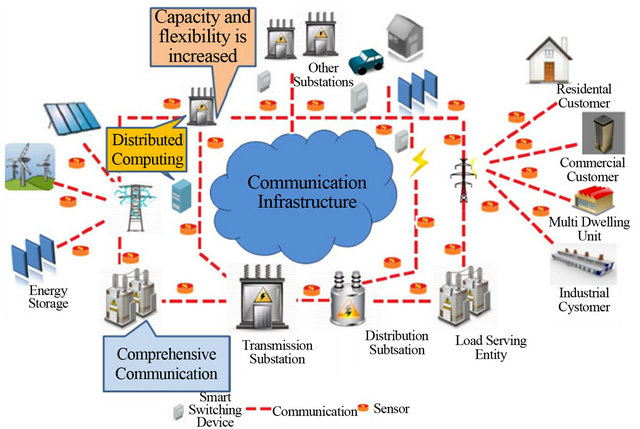
\includegraphics[totalheight=6cm]{smart_grid_infrastructure.png}}
    \caption{Smart grid architecture increases the capacity and flexibility of the net- work and provides advanced sensing and control through modern communica- tions technologies \cite{gungor2011smart}}
    \label{fig:mesh}
\end{figure}

\textbf{Data generated from smart grids: Delete this line after completing}

Apart from increased efficiency, self-restoration, operation automation, and renewable energy integration, the smart grids are potential sources of big data. The information technology support for the power transmission and distribution produces rapid amount of data. The sensors, the smart meters, the control units and the monitoring devices all add up to this huge volumes. Data are generated from various activities such as: power utilization habits of the users; phasor measurement data for situational awareness; energy consumption data measured by the widespread smart meters; energy market pricing and bidding data collected by advanced metering infrastructure; management, control and maintenance data of devices and equipment in the power generation, control data exchanged between transmission and distribution networks acquired by intelligent electronic devices \cite{lai2015big}. 

The grid is becoming more and more digital with the information recorded by the sensors and the smart meters deployed at the users' premises and along the grid and power stations. This data can be for example, consumption data from smart metering and electric vehicles, data telling about the conditions of the components in the grid \cite{aiello2014smart}. For achieving fine-grained monitoring and scheduling, information from the power grid needs to be collected within short intervals. 

\textbf{Energy saving using Smart grids}
\textbf{Effects of data, why are they collected : Delete this line after completing}

Collecting and managing, processing and analyzing electrical data reveals deeper insights that can help experts to improve the operation of power grid to achieve better performance. The technology to collect massive amounts of data is available today, but managing the data efficiently and extracting the most useful information out of it remains a challenge. Data obtained from the smart grids provides valuable information which helps for efficient grid operations. It is also closely related to the safety and reliability of the power system operation and management based on data-driven decision support. Using data from meters and sensors, an operator could be alerted that a transformer is having problems and help to make a decision from the information provided. For example, in the past when a transformer would fail, the lights would go out and the operator only knew about it when customers called. In future we would wish to have a sensor on the power line which sends an alert to the operator about that transformer. The operator recognizes where the outage is and dispatches a person to fix the problem. This gets the lights back on sooner and results in more satisfied customers \cite{Troiano}. 

With this technology, electrical utilities are equipped to deliver power more efficiently, improve operations, reduce emissions and management costs, and restore power faster. And operators are able to immediately identify outages, allowing for improved efficiency to manage responses. Smart grid data could also generate information on how individual customers respond to requests of consumption reduction. It is also possible to use real-time metering data to discover unaccounted consumption when energy is being diverted and stolen, reducing the cost of distribution operations. With smart meters, utilities can learn about the information of the number of units consumed by the user and the state of the grid. This information allows the power grids to deploy optimization techniques to find the optimal power generation, control mechanisms and transmission strategies for that state of grid.

 Construction and application of the smart grid have stimulated the accumulation of electric power grid operation data, production management data and electricity consumption data \cite{chen2016data}. The accumulated data contain redundant, missing and outlier data, resulting in serious issues of electric power data quality.  These electrical data can be used by data analytics researchers to obtain patterns and to make better decisions for electric utilization and control. They can make use of several techniques, including statistics, clustering algorithms, data mining, machine learning, signal processing, pattern recognition, optimisation and visualisation method to capture, curate, analyze and visualize the data. 

As there are advancement in technology, there are adverse effects as well. Over the last years power grids have been targeted with hazardous malware to steal their data and get access to their communication. Security is one feature which plays a very huge role in every communication entity. Since smart grids and the power generators exchange informations, intrusions, attacks and anomalies could occur because of malware activities. In order to accomplish these security goals we propose to use techniques which will be discussed in the later sections.

\begin{figure}
\centerline{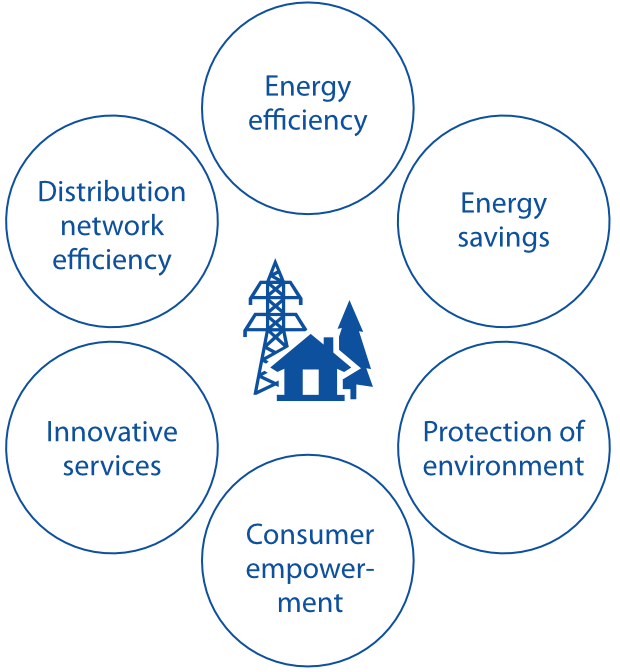
\includegraphics[totalheight=6cm]{SM_benefits.png}}
    \caption{Six ways the adoption of smart metering systems can benefit the electricity customer. 
    {Image src: http://www.foxconngfo.com/iot/foxconn/page-11.html}}
    \label{fig:SM_Benefits}
\end{figure}


\textbf{Our proposal for nullifying one of the effect: Delete this line after completing}
The massive amounts of measurement data that will be made available at distributed locations that can and must be leveraged to optimally operate the power grid.


\textbf{Added Newly: Should i write about how electricity is produced and transmitted, what are the tradeoffs to be considered when deploying the anomaly detection algorithms in the smart grids. }

In order to efficiently utilize the energy it requires one to study detailed knowledge of the energy usage patterns of the locations. For this we consider the energy usage patterns of the locations in order to identify irregularities of the transmitted energy. We do this by detection algorithms using the modern machine learning techniques. Apart  from  the  economic  benefit  brought along by the increased energy efficiency, there is also an urgent global need to reduce carbon emissions such as carbon dioxide,  which is closely tied up with the generation and hence consumption of electricity \cite{chan2012load}. Generally,  this  can  be  reduced  by  using  clean  (or cleaner) energy sources and the control of electricity consumption  or  demands  at  the  users’  side.
	The main aim of smart grids are to provide \begin{itemize}\item more efficient transmission of electricity. \item quicker restoration of electricity after power disturbances. \item reduced operations and management costs for utilities, and ultimately lower power costs for consumers. \item reduced peak demand, which will also help lower electricity rates. \item increased integration of large-scale renewable energy systems. \item better integration of customer-owner power generation systems, including renewable energy systems. \item improved security. \end{itemize}

Nevertheless, increased interconnection and integration also introduce vulnerabilities into the grid. Failure to address these problems will hinder the modernization of the existing power system. Through advanced sensing technologies and control methods, smart grids can capture and analyze data regarding power usage, delivery, and generation in near real-time. According to the analysis results, the smart grid may provide predictive information and corresponding recommendations to all stakeholders (e.g., utilities, suppliers, and consumers) regarding the optimization of their power utilization. It may also offer services like intelligent appliance control for energy efficiency and better integration of distributed energy resources (DERs) to reduce carbon emissions. Apparently, it is not a simple grid in the sense of our current power grid. It can be regarded as a “system of systems” that involves both information technology (IT) and electricity system operations and governance. Such a complex system undoubtedly presents many challenges, especially in cyber security and privacy aspects \cite{liu2012cyber}.

Smart grids should also consider the wide range of needs and power quality requirements. Power quality involves factors like voltage flicker, voltage volume, momentary interruptions, etc. Different consumers may have distinct power quality requirements (e.g., industrial vs. residential users). Optimizing the distribution of power by detecting the irregularities, outliers or anomalies will reduce power consumption. These timely detection of faults by using the proposed technologies will help in operating resiliently to disturbances, attacks and Natural disasters. Gann et al.  affirmed that cities become “smarter” when they exploit the increasing data and analytical techniques available, in order to improve energy effectiveness and efficiency through the integration of physical infrastructures and digital technologies \cite{gann2011physical}

\textbf{end}


The energy grid can now interact with the end user to control his energy consumption, by either direct control on some of his appliances (for example, the washing machine) or indirect control, by providing fine grain resolution on the cost of the energy at a given day and time, such that the final user tunes up his own schedule for the energy consumption. The grid can also promote cooperation among different prosumers (both producers and consumers of energy) to enable more efficient energy usage, particularly in what concerns consuming on the spot for renewable energies.

Discovering new information can be very beneficial to both power distribution grids and customers. Uncovering hidden energy usage patterns, identifying untapped energy efficiency opportunities, engaging customers for demand response programs by discovering high usage patterns, for instance, inefficient thermostat setpoints and charging their electric vehicles, can save a lot of energy and expenses of the customers \cite{ben7utilities}. 


Data is the fundamental currency of the smart grid. A clear understanding of how these data are generated, what it consists of, and the benefits it can be used to deliver is critical to realizing the fullest possible returns from smart grid investments. The benefit is to have enriched information of the performance of the system, its stability, and customer consumption. For this task, anomalies are of special interest, because they can be caused either by faulty equipment or potentially misconfigured devices consuming significantly more or less energy than required for proper operation.


Complex electric power system contains large amounts of real-time data. Data is accurate or not, which determines the safety and reliability of electric power system. Outlier data may affect the normal operation of electric power system and even threaten the security of entire system. Hence, in order to ensure the stable and safe operation of electric power system, it has important significances to extract and detect these outlier data from the original data. The significances of electricity consumption outlier data have two aspects on negative and positive influences.

The negative influences include the following aspects. Firstly, the presence of electricity consumption outlier data will reduce the accuracy of assessment. Then, the results of data mining cannot accurately reflect the characteristics of data. Finally, outlier data affect the judgement and decision of electric power system dispatcher \cite{huang2004enhancement}. It even threatens the safe operation of system. If outlier data cannot be correctly identified and effectively corrected, they will provide false prediction as a reference \cite{pham2014anomaly}. This affects the accuracy and reliability of prediction results. Furthermore, if outlier data are used as modeling data, it will interfere with the changing rules and influence the training accuracy. If outlier data are used as a predictor of test results, it can lead to erroneous judgement \cite{mao2005principle}.

Outlier detection of electricity consumption data is to find out the relatively sparse and isolated outlier data patterns which are hidden in massive data \cite{chen2016data}. In the early stage of data set preprocessing, we usually put outlier data as noise data. Although outlier detection finds the hidden data in the data set as the main purpose, outlier data mining is more valuable and meaningful than other types of mining [70]. Because one hundred thousand normal records are likely to cover only one rule, but ten outlier records are likely to cover ten different rules \cite{mao2005principle}, \cite{chen2016data}. Outlier detection of electricity consumption data may provide us more important information, so that we can find some real and unexpected knowledge, which can help us to understand the consumer behavior, capture the theft, find system vulnerabilities and failures and improve service quality \cite{pham2014anomaly} .

There is a growing interest in understanding how energy is spent in the commercial buildings. Furthermore, distributors of electricity want to know how to reduce the failure rate and detect anomalies which will serve the purpose of reliability and efficiency of the smart grid. In addition, they want to know how to visualize large volumes of energy data collected by power meters (sensors) in a building to find patterns, trends, and anomalies. In the end, our goal is to find how to automatically discover the anomaly, like unusual power consumption measurements highly differing from old observed patterns, and to reduce the energy cost of a building. For this task, anomalies are of special interest, because they can be caused either by faulty equipment or potentially misconfigured devices consuming significantly more or less energy than required for proper operation \cite{janetzko2014anomaly}.

\frenchspacing Vulnerabilities in power systems can cause a major disaster considering the large usage of electricity in today's world. A widespread loss of power even for few days, could make devices ranging from cellphones to ATMs to traffic lights, and even lives to halt, if heating, air conditioning and health care systems exhaust their backup utilities. But when dealing with infrastructure that may even be system-critical, the number of failures must be reduced to an absolute minimum. Early signs of failures should be visible in power usage patterns \cite{janetzko2014anomaly}. By detecting anomalies in the usage patterns of electricity, machine learning algorithms can help utilities take customer care a step further, helping them identify homes at greatest risk of switching providers, listen to their concerns, and offer solutions. Our motivation therefore, will be concentrated on finding the appropriate information from the collected smart grids data and to employ suitable discovery method on these data to detect vulnerabilities and/or anomalies in the data. 

\frenchspacing

\label{sec:Introduction}

\chapter{Research questions and Challenges}
Smart Grid generates a significant amount of data due to large scale deployment of digital technologies in distribution network on a daily basis, and these data must be processed in an efficient way in order to monitor the operational status of the grid. Research has shown that many existing techniques in the field of data analytics have not fully explored the value of data. However, serious attention has been given to this field and some well-known institutions have updated their teaching and research programs to higher education students who can take up the challenges of big data research and applications in the near future. Data analytics competitors are competing to bring a set of IT tools and capabilities that are largely new to the utility industry \cite{lai2015big}. 

Information is necessary for energy players, and for decision-makers and regulators who must establish rules and mechanisms to provide a framework for a competitive market and allow smart grids to achieve optimal efficiency \cite{clastres2011smart}. With the worldwide initiative of upgrading the traditional electrical grid to the Smart Grid, new challenges have been introduced, among which is the “Big Data” challenge. Many researchers are asking themselves what they can do to harness this deluge of data to make more intelligent operational and business decisions. 

With smart grids, it will be possible to obtain accurate, real-time data on consumption profiles and the status of electricity systems, with scope for isolating certain items on which it is appropriate to act (heating, household devices, etc.). Measures to promote energy efficiency and control consumption will benefit from the new behavioural data. The positive effect expected of smart grids is not necessarily a drop in prices but rather a reduction in the bills paid by consumers. It is estimated that gains from optimizing or reducing consumption will counterbalance higher prices due to regulation of and higher security on the electricity system\cite{clastres2011smart}. 

Regarding data analytics applications to the smart grid, the key challenges are focused on converting the tens of billions of data points coming from the millions of smart meters deployed around the country and turning them into actionable information for the grid operations. The data could generate information on how individual customers respond to requests of consumption reduction. It is also possible to use real-time metering data to discover unaccounted consumption when energy is being diverted and stolen. The aim is to improve grid reliability, outage response and reducing the cost of distribution operations. Occasionally emerged frauds or intrusions in smart grid systems have incurred significant loss when the suspicious activities were not detected or inefficiently processed. Therefore we found some of the research questions and challenges which needs to be answered to efficiently deploy the anomaly detection methods for electrical data:

\begin{enumerate}
\item \textbf{Availability of sufficient and valid input data:} For any machine learning algorithms to work and perform with good accuracy, is dependent on the size of input data. Sufficient amount of data will provide us with prior knowledge about the relationship between the variables, without which it will be difficult to generalize the unseen data. In our case of predicting unexpected events, working with small set of data could be challenging, as we may not capture required dependencies between the variables in the data, given the data is not large enough. We limit ourselves to only the size of the data in this discussion and won't be discussing about how the data is collected, assuming it is collected efficiently and systematically. It is important to know what is the data used for analysis, keeping in mind the purpose of the data and about the learning outcomes of it. Next, how many data points are enough to provide the evidence of the outcome achievement. Further details of how much data is enough can be found in \cite{rogers2002death}

\item \textbf{Dealing with unlabeled data:} The electrical data used for our analysis do not contain labels for anomalies and hence we use the general term "unlabeled data" as used in machine learning. We proceed by considering that most part of the data contain normal patterns and only a small part contain anomalous patterns. This assumption will be proved right or wrong later in the evaluation section after modeling and training the data. There is no explanation for each piece of data, it just contains data and nothing else. Challenge arises in determining which data to be considered as normal and which data as anomaly since we do not have labels or classes to distinguish. Dealing with unlabeled data also challenges the choice of algorithm to be implemented which works the best with these data. Sometimes it can be taken into account that the accuracy in prediction will be high when using enough amount unlabeled data than labeled data \cite{liang2007use}.

\item \textbf{Identifying useful information:}The next challenge arises is feature selection. Identifying only the relevant features is important part of machine learning in anomaly detection. We need to take care of removing unnecessary data such as duplicates in the data which may be caused due to inefficient measurements and data containing 'null' values. Cleaning the data for removal of duplicates, null values and also to remove noise will help to analyse the data efficiently. Data Smoothing, by considering moving average windows readily available in python libraries can be used to do this cleaning process.

\item \textbf{Dimensionality Reduction:} Dimensionality reduction is used as an efficient technique when considering high dimensional datasets. Our anomaly detection process will be hard if we do not consider reducing the data to low dimension. To retain all the necessary information without losing any important aspects of the data will be challenging. For this we will employ well known dimensionality reduction machine learning technique such as PCA. PCA will reduce the dimensionality in the data considering only relevant information representing the whole data and ignoring the information which do not effect our anomaly detection process and which do not lose any important information about the data.

\item \textbf{Determining a suitable model of normality:} How to model the data will be the biggest challenge in our work. Modelling the data will determine the performance of the process of detecting the anomalies as well to describe the process efficiently. Model which best suit our data should be utilized. We will start with the basic and well known Gaussian Mixture Models and then PCA with residual parameters, followed by one of the efficient deep learning model, LSTM (Long Short-term Memory).
 
\item \textbf{Train the model:}Simply turning the work over to machines won’t help: most machine learning and statistical mining techniques also hold the assumption that historical data, which is used to train the machine-learning model, behaves similarly to the target data, to which the model is later applied. We should be able to determine, what is the percentage of data to be used for training, validating and testing the model. The training data should be able to capture all the necessary features of the data which will be used to predict the future events. Choosing the training data will directly effect the accuracy of our model, 

\item \textbf{Finding optimal model parameters:}  Identify suitable statistical metric with which we will prove the correctness of our model. This statistical metric should be able to calculate the threshold with which our model distinguishes between normal and abnormal patterns. This threshold value will the borderline between normal behavior and anomalous behavior. Choose a proper threshold above or below which data can be considered as anomaly/ies. Measures have to be taken care while fitting the model. A good model for the data should not overfit by using very large model parameters and it should not underfit as well using very less model parameters. Determining proper model parameters to include huge amount of data poses challenges to avoid the number of false positives and false negatives. False positives are data which are detected as anomalous are not truly anomalous and False negatives are data which are anomalous but our model did not detect.

\item \textbf{Deployment Efforts:} Great efforts have to be spent to develop more advanced and efficient algorithms for data analysis. Training the model with sufficient data, validating it and testing our methods consumed the most part of our work. 
\end{enumerate}
\label{sec:Research questions and Challenges}

\chapter{Related Work}
A report on smart grid data management by analytic researchers at Accenture discusses five different data classes for smart grids in \cite{analytics2010achieving}: 
<Churn-rate> : in its broadest sense, is a measure of the number of individuals or items moving out of a collective group over a specific period of time. It is one of two primary factors that determine the steady-state level of customers a business will support.
\begin{enumerate}
 \item \textbf{Operational data}: Represents the electrical behavior of the grid. It includes data such as voltage and current phasors, real and reactive power flows, demand response capacity, distributed energy capacity and power flows, and forecasts for any of these data items.
\item \textbf{Non-operational data}: Represents the condition, health and behavior of assets. It includes master data, data on power quality and reliability, asset stressors, utilization, and telemetry from instruments not directly associated with grid power delivery.
\item \textbf{Meter usage data}: Includes data on total power usage and demand values such as average, peak and time of day. It does not include data items such as voltages, power flows, power factor or power quality data, which are sourced at meters but fall into other data classes.
\item \textbf{Event message data}: Consists of asynchronous event messages from smart grid devices. It includes meter voltage loss/restoration messages, fault detection event messages and event outputs from various technical analytics. As this data is triggered by events, it tends to come in big bursts.
\item \textbf{Metadata}: Is the overarching data needed to organize and interpret all the other data classes. It includes data on grid connectivity, network addresses, point lists, calibration constants, normalizing factors, element naming and network parameters and protocols. Given this scope, managing metadata for a smart grid is a highly challenging task. 
\end{enumerate}
Outlier data have an important influence on accuracy, completeness and self-consistency of data quality. At the same time, it has important events information of electric power grid, such as power rationing, equipment failures and so on \cite{zhang2005new}. Thus, it is of great significance to identify, analyze and deal with outlier data. In residential or industrial electricity, it will produce large amounts of consumption data. Most consumption data are normal. However, there are also some outlier data. The generation of outlier data usually has the following reasons.
\begin{enumerate}
 \item
When electric power system is in operation, measurement and transmission processes of data acquisition system may generate outlier data. For example, outlier changes of data in the transmission are caused by the failure of data transmission system \cite{xu2014application}. Thus, data may lose or confuse in the transmission process.
 \item
The data acquisition system is normal. But outlier changes of electric load are caused by special events, such as: line outage maintenance \cite{dasu1999hunting}. The occurrence of special events usually makes the electricity consumption data in a certain period of time as a null value. This is a kind of outlier phenomenon.
 \item
Significant electricity reforms make electricity consumption habits changed, such as: Ladder-type price \cite{yu2011detecting}. Ladder-type price sets a base to residents, and more than the base price will increase the electricity price. This will lead to changes of electricity habits and result in outlier electricity consumption.
 \item
These conditions may also produce outlier data, such as: records errors, artificial forgery and so on. User's electricity consumption data may hide the user's electricity behavior habits. For data mining of electricity consumption data, on the one hand, it can understand the users’ demands for personalized service; on the other hand, it can detect the users’ stealing behavior and protect the benefits of enterprises.
\end{enumerate}
\frenchspacing 
Applying data mining techniques for power consumption data is a known approach for identifying abnormal usage behavior. Agarwal et al. examined 6 months of data from the UCSD campus, including aggregate power consumption of four buildings in \cite{agarwal2009energy}. Agarwal et al. focuses more on the setup of power meters and provide only simple visualization methods like line charts. Catterson et al. used an approach to monitor old power transformers in \cite{catterson2010online}. Their goal is to proactively search for abnormal behavior that may indicate the transformer is about to fail. Similarly, McArthur et al. searched for anomalies to detect problems with power generation equipment in \cite{mcarthur2005agent}. Jakkula and Cook compared several outlier detection methods to find which is better at identifying abnormal power consumption in \cite{jakkula2010outlier}. J Seem used outlier detection to determine if the energy consumption for a day is significantly different from previous days’ energy consumption in \cite{seem2007using}. This is a known approach for identifying abnormal system behavior.

\frenchspacing There has been many work which already concentrates on securing the smart grid against the cyber- security threats. Rajasegarar et al. discusses anomaly detection techniques in wireless sensor networks considering the limited resources and their effects in \cite{rajasegarar2008anomaly}. Zhang et al. proposes a distribution intrusion detection system which developed and deployed intelligent and multiple analyzing modules in different layers of the smart grid in \cite{zhang2011distributed}. These systems uses support vector machines and Artificial immune systems to detect and classify possible cyber attacks. Fadlullah et al. and Gellings et al. have made steps towards machine to machine communications in [\cite{fadlullah2011early},\cite{gellings2009smart}]. Fadlullah et al. discusses early warning detection technologies in smart grid communication using Gaussian process. With this warning system in place the smart grid control center can forecast the malicious activities to the smart grid which helps it to take measures against such activities. Perl et al. also proposes a solution to outlier detection using Gaussian Mixture model in \cite{perl2009outlier}. 

Ozay et al. uses the machine learning algorithms to detect and classify the measurements as secure and non secure in \cite{ozay2015machine}. It includes well known batch and online learning algorithms (supervised and semi-supervised). It takes advantage of the relationship between the statistical and geographical properties of the attack vectors. These properties are used to detect the unobservable patterns in the attacks. Janetzko et al. describes an analytical and visual approach in detecting anomalies and examining energy consumption data in \cite{janetzko2014anomaly}. The goal of the research was to enable the analyst to understand the power consumption behavior and to be aware of unexpected power consumption values. 

For anomaly detection, machine learning techniques are often applied for detecting security threats, such as data injections or intrusions, instead of detecting bad data measurements. The latter is usually addressed by developing PMU placement algorithms that allow measurement redundancy [\cite{chen2006placement},\cite{tarali2012bad}]. Hink et al. evaluated various machine learning methods to differentiate cyber-attacks from disturbances \cite{hink2014machine}. These methods include OneR, Naive Bayes, SVM, JRipper, and Adaboost. Among these approaches, the results show that applying both JRipper and Adaboost over a three-class space (attack, natural disturbance, and no event) is the most effective approach with the highest accuracy. Pan et al. propose a hybrid intrusion system based on common path mining \cite{pan2015developing}. This approach aggregates both synchrophasor measurement data and audit logs. 

In addition, SVMs have also been used in detection data cyberattacks. For instance, Landford et al. proposes a SVM based approach for detecting PMU data spoofs by learning correlations of data collected by PMUs which are electrically close to each other \cite{landford2015fast}. Due to the time sensitivity of event and anomaly detection on the Smart Grid, a major challenge of applying machine learning techniques to perform these tasks is the efficiency of these approaches. This is especially important for online detection of events. Two different types of approaches have been used to address this challenge. Dimensionality reduction is a commonly used approach to improve learning efficiency by reducing the complexity of the data while preserving the most variance of the original data \cite{van2009dimensionality}. A significant amount of efforts have been made in this direction. For instance, Xie et al. propose a dimensionality reduction method based on principal component analysis for online PMU data processing \cite{xie2014dimensionality}. It has been shown that this method can efficiently detect events at an early stage. A similar technique is used to reduce the dimensionality of synchrophasor data by extracting correlations of the data, and presenting it with their principal components in \cite{dahal2012online}. 

Gaussian Mixture Models have been used extensively in fault detection techniques. Fulufhelo et al. have used GMM classifier in conjunction with the Melfrequency Cepstral Coefficients (MFCC) and Kurtosis features for bearing fault diagnosis in \cite{nelwamondo2006faults}. Detection of a defect in bearings is a process of classifying any of the obtained vibration signals into classes that have been defined during the model generation stage. Li et al. detect unusual patterns in flight data using GMM and is done in \cite{li2016anomaly}. They start transforms the digital flight data into a form applicable for cluster analysis, cluster analysis with a Gaussian Mixture Model (GMM), which characterizes typical behaviors of aircraft systems and temporal patterns of flight operations, detects anomalies based on the norm established in the previous step, safety experts review these anomalies to identify any safety risks at stake.

Li et al. uses probability density function as the measure to detect anomalies which is similar to our approach instead we use weighted log probabilities and an efficient threshold to detect anomalies. A probability density profile for every flight is being constructed after calculating the pdf of every data sample. Abnormal samples are detected by identifying samples with probabilities that is lower than a threshold. This threshold value is associated with the sensitivity of the detection system, and can be adjusted based on the distribution of all samples in a dataset.

Laxhammar et al. also uses GMM and adaptive Kernel Density Estimator to detect anomalies in sea traffic \cite{laxhammar2009anomaly}. The models and algorithms proposed for anomaly detection in the maritime domain are more or less data driven in the sense that normalcy is determined by machine learning algorithms analyzing a relative large set of historical data assumed to reflect normalcy. Anomaly detection results for both models were quite disappointing as the expected trajectory distance observed before detection was considered rather large given the rather constrained normal trajectories and the sweeping and stochastic character of the anomalous trajectories.
\label{sec:related}

\chapter{Understanding Electrical Data}
As machine learning techniques have become the de facto approaches for Big Data analytics, these techniques are also applied and adapted to process and analyze electrical data. A common objective of the electrical data analysis is to recognize and identify patterns, or signatures of events that occur on the Smart Grid. Therefore, a large number of these approaches are based on pattern recognition \cite{al2012synchrophasor}.Finding pattern or recognizing pattern can be considered as fitting a model in the data. Such an outcome is the result of a cascaded work process namely preparing data, searching pattern, evaluating knowledge and finally referring it towards the monitoring and control units. We look at each of this briefly to understand the data thoroughly before diving into anomaly detection methods. We visualize our data, looking for inital ideas in determining patterns of electrical data using state of art machine learning libraries. 

Data preparation includes data cleaning, data integration and transformation, data reduction and data warehousing which will explained in detail below. Before diving deep into understanding the data process-by-process, what we might learn from the dataset includes:

\begin{itemize}

  \item The number of records in the dataset
  \item The number of attributes (or features)
  \item For each attribute, what are the datatypes(nominal, ordinal, or continuous)
  \item For nominal attributes, what are the values
  \item For continuous attributes, the statistics and distribution
  \item For any attributes, are there any missing values
  \item For any attributes, the number of distinct values

\end{itemize}

\begin{enumerate}
\item\textbf{Preparing Data:} Machine learning algorithms learn from data. It is critical that we feed them the right data for the problem we want to solve \cite{brownlee2013prepare}. Even if we have good data, we need to make sure that it is in a useful scale, format and even that meaningful features are included. This data preparation process has direct impact on the result, the more discipline we are in handling the data, the more consistent and better result we will able to achieve. Below are the three important data processing steps widely followed when using machine learning algorithms, namely:
	\begin{enumerate}
		\item\textbf{Selection of Data:} Our dataset is a collection of huge volumes of electrical distribution measurements. Identifying patterns by running through all this data is time consuming, so we consider subsets of it for our analysis. The subsets are carefully chosen so that we may not miss out important information related to identifying anomalies. The data obtained is measured by sensors deployed across the distribution network and this data is available for the wholeday read around every second. Hence we have 24*60*60 = 86400 observations for a complete day, so by taking one or two weeks of data in the form of two different sets (weekday data of normal working days and weekends data following the normal working days) without any holidays from a particular region would be good and big enough to be assured of not missing any relevant information. 
		\item\textbf{Preprocessing Data:} We now have selected data which needs to be preprocessed before we can apply anomaly detection methods. The performance of anomaly detection methods depends vastly on how clean the data is, do we need to format the data and is there any noise data in it. Cleaning the data is removal of redundant values which we can see by looking at the data or by fixing the missing data. In our electrical data, we have values such as energy transported and energy consumed which contain previous day values along with currently measured value which is not necessary for anomaly detection. Likewise we have reactive current values which are available for few regions and not available in few, therefore we can remove these missing and non-important data. In order to remove the noise we can use data smoothing techniques which will be discussed later.
		\item\textbf{Transformation of Data:} We have selected the dataset which is big enough, cleaned and formatted the data which looks good for analysis but, in order for the machine learning algorithms to fit the data to the proposed model we need to transform the data accordingly. One method which plays very important role for our anomaly detection process is scaling. We have mixture of values in our dataset like, voltages, current, power, phase displacement which are measured on different scales( volts, amperes, watts, degree) and hence bringing these values under one common scale can prove beneficial for our detection process. Principal Component Analysis(PCA) is yet another technique which transforms the data such that the data are represented according to the variances. Its a very useful statistical method widely used in machine learning for reducing the dimensions of the data. We have even proposed the detection of anomaly method using PCA in our work which will be discussed in detail later. Likewise we can also use data decomposition and aggregation when necessary. 
	\end{enumerate}



\item\textbf{Searching Patterns in the data:} Our next step in understanding the data is finding about the patterns in the data. Several statistical methods are already readily available which we will leverage for working with our electrical data. Some of the methods which we believe would be an asset in finding the patterns in our electrical data are briefly discussed below:
\begin{enumerate}
\item\textbf{Correlation:} Correlation is a statistical technique which tells you how variables in our dataset are related. A simple correlation plotted against our set of electrical data is as shown in the figure \ref{fig:correlation}. We have used the existing correlation method available under python pandas library. It computes the \textit{pearson} correlation coefficient which is the default correlation method available along with \textit{kendall} and \textit{spearman}. The details of these methods are not covered here, as it is out of scope of our work. The correlation measure as in the figure provides us with initial information about which features to consider and which features will not be so useful in finding the patterns. The correlation matrix is calculated across each column of our dataset. Some important observations are, variables which are directly related have high correlation values meaning, an increase in the value of one variable increases the corresponding related variable and similarly a low correlation value means the two columns are independent of each other. 

\begin{figure}[tph!]
\centerline{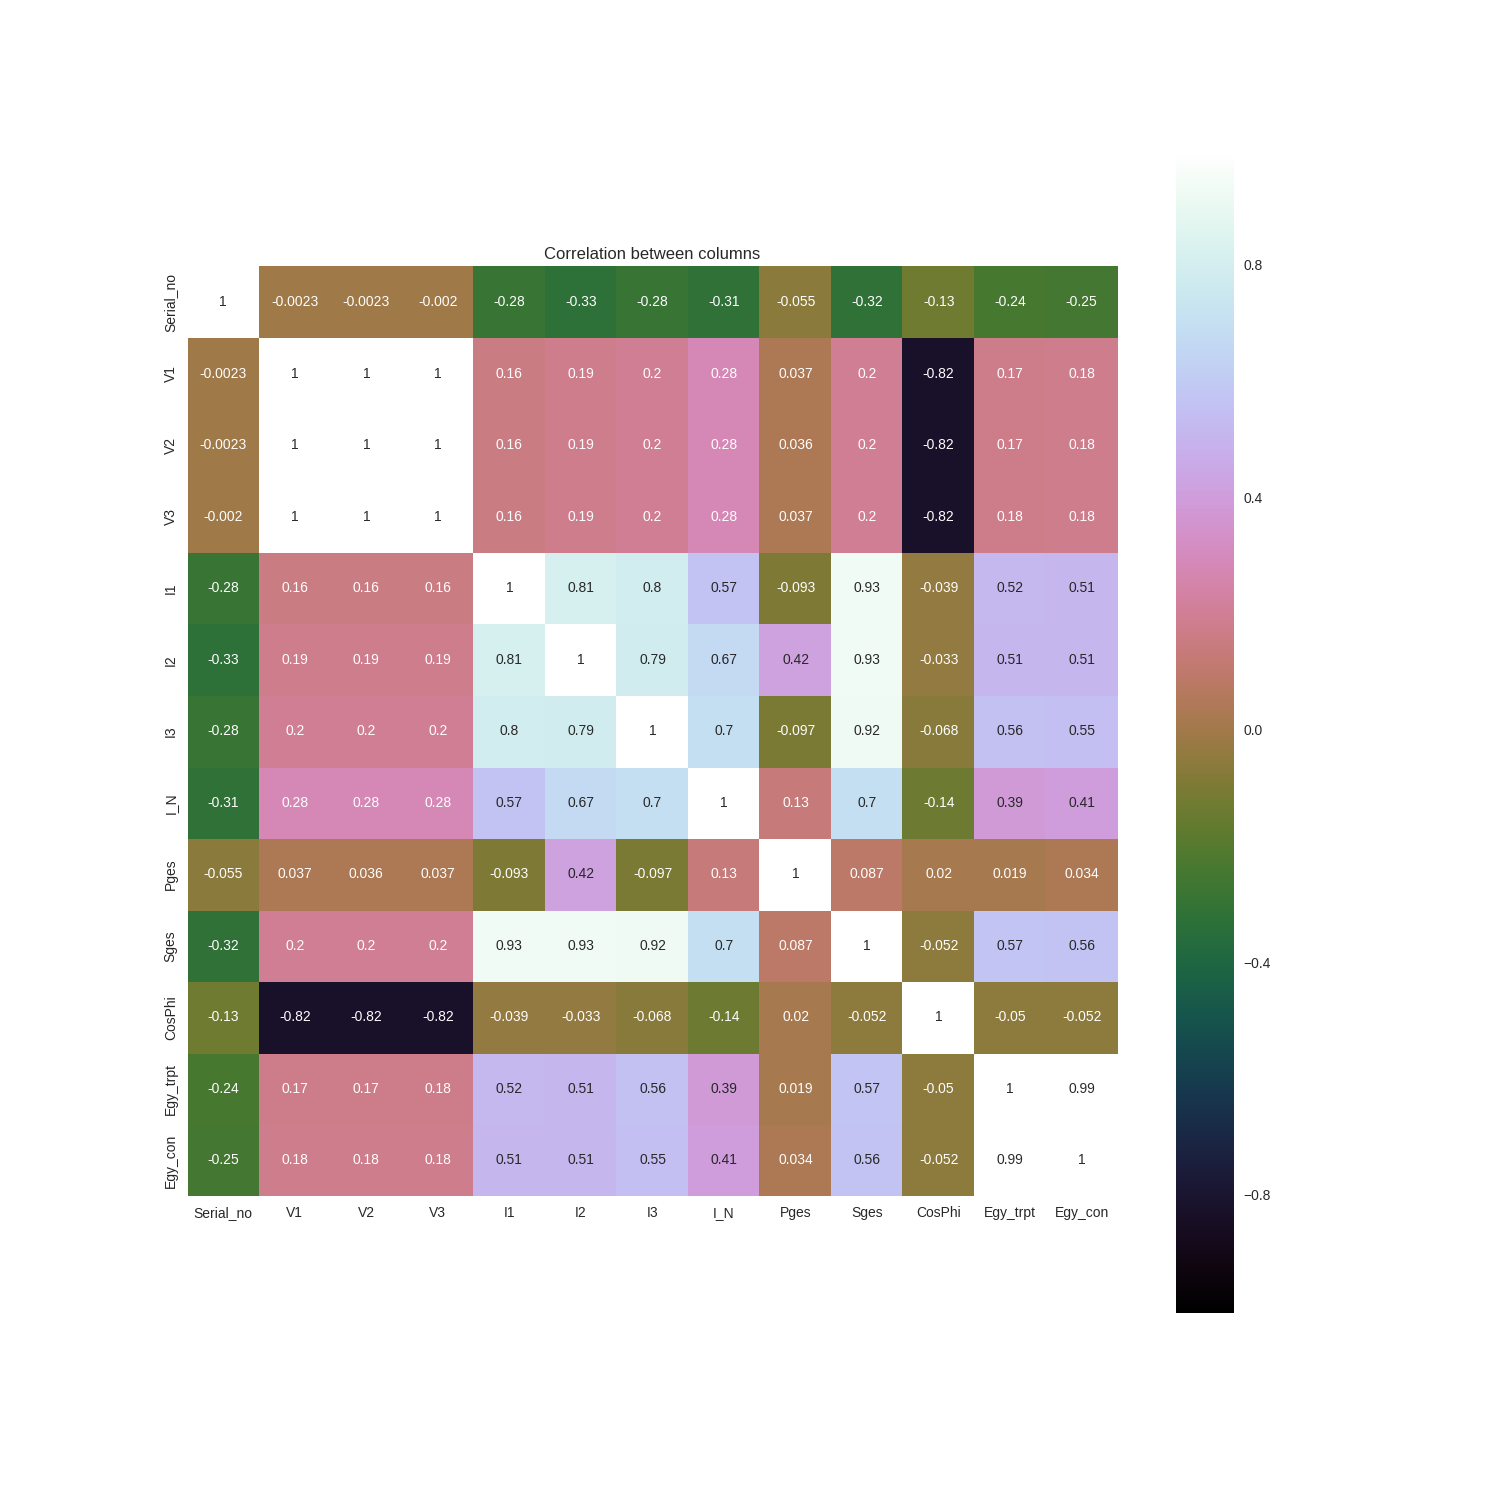
\includegraphics[totalheight=10cm]{Correlation.png}}
\caption{Correlation matrix of Data}
\label{fig:correlation}
\end{figure}
A positive correlation indicates the two columns behave similar that is, for two positively correlated variables 'a' and 'b', the value of 'b' increases with increase in 'a' and correspondingly decreases with decrease in 'a'. A negative correlation is vice versa, increase in value of 'a' decreases 'b' and decrease in value of 'a' increases the value in 'b'.  A correlation value of 1 and closer to 1 are said to be highly correlated, as you can see the diagonal elements in the figure all have values 1 which means the column values are highly correlated among themselves, while the column variables representing voltages seem to have very less correlation with current and power consumed/transported  values. Such less correlated values can be considered as potential columns for our analysis in finding the anomalies as these values are independent of each other. We concentrate on these low correlated columns and believe highly correlated values are not so important for our research.

\item\textbf{Histogram:} Histograms are another way of visualizing the data to get the initial look of how our data is distributed. For continuous variables as in our case, a histogram can be used to assess the spread and shape of our data and suits particularly well when we have large number of observations. Bins in the histograms define the width of the class intervals, with sufficient number of bins, histograms will provide the peak and unusual data details. A simple histogram plot for our dataset which has been normalized to mean=0 and variance=1 is as shown in the Figure \ref{fig:hist1}. We can see that the data is following a normal distribution with the tails distributed on either side of mean and in between -5 and +5. We can also deduce from the Figure \ref{fig:hist1} that the data points are likely to occur mostly near the mean and the occurence of points decreases on both sides of mean and becomes more less probable. This means that a value which tends to move very much further away from the mean will be less probable and can be considered as outlier in our distribution. 
\begin{figure}[tph!]
\centerline{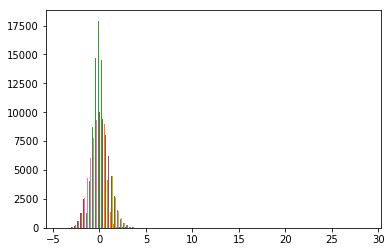
\includegraphics[totalheight=6cm]{histogram.png}}
\caption{Histogram of the data}
\label{fig:hist1}
\end{figure}
\item\textbf{Box and whisker plot:} Till now we have considered techniques which make use of the entire columns. Let us look at single column and check how the values in each column look like. We can get to know what is the maximum, minimum and mean value of each column by using box and whisker plots. The plot displays some important information for instance, the range, median and quartile, which reflects the actual data. It is yet another technique used in exploratory data analysis, a numerical detective work which uncovers the possibility of quantitative interrelationships among the data \cite{larsen1985box}. The box and whisker plot of first 100 values of Voltage V1 is as shown in the Figure \ref{fig:boxplot}. Among the 100 values, the topmost point in the figure shows the maximum value, the bottommost point shows the minimum value. The topmost and the bottommost points are called whiskers, the rectangle has the lower and upper quartile constituting inter-quartile range and the median is represented by the orange line inside the rectangle. This gives us the idea of how the column values are distributed numerically. The points  which lies outside 3 times of interquartile range can be suspected to be an outlier or an anomaly point.
\begin{figure}[tph!]
\centerline{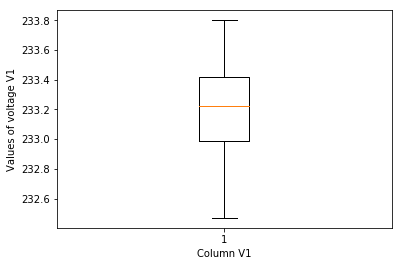
\includegraphics[totalheight=6cm]{Boxplot.png}}
    \caption{Box plot of first 100 values of Voltage V1 }
    \label{fig:boxplot}
\end{figure}
\item\textbf{GGplot:} Another useful visualization tool for identifying relationship between column values in our data is ggplot. GGplot does this by mapping the values of two columns against each other. We can view this as an alternative approach to correlation but, with the distribution of points. Correlation matrix will give you the measure of how two column values are related by a numerical value between 0 and 1, while ggplot will help you visualize the column values individually in the form of scatter plot and aid the process of understanding the electrical data in much easier way. We have plotted voltage value V1 against the phase displacement value CosPhi in the Figure \ref{fig:ggplot}. We can make a conclusion that most of the values of voltages are within the range of 225 and 240 volts, whereas the CosPhi values are within the range of 0.75 to 1. The values very far from this range can be considered as unusual.
\begin{figure}[tph!]
\centerline{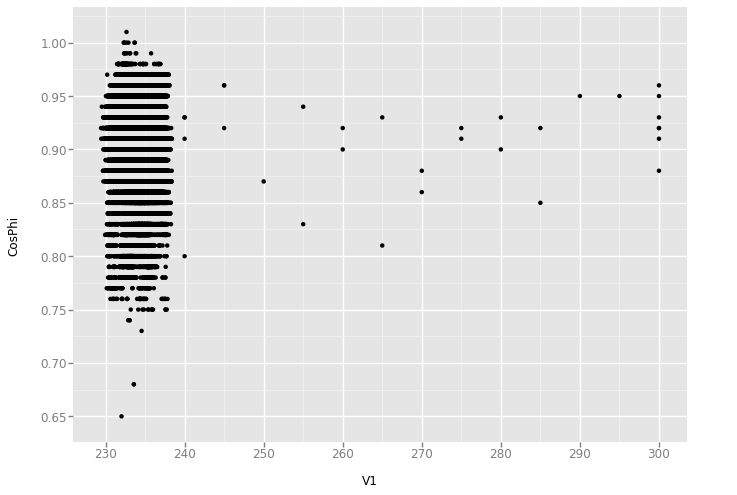
\includegraphics[totalheight=6cm]{ggplot_V1_CosPhi.png}}
\caption{ggplot of Voltage versus Phase Displacement.}
\label{fig:ggplot}
\end{figure}
\end{enumerate}
				
	
\item\textbf{Knowledge Discovery:}




\item\textbf{Evaluating against the goal:}
\end{enumerate}
In order to visualize the huge set of electrical data collected from electrical grids we had to store all the data in a database. Storing the data into the database will not only allow us to compute the statistics better but also, will enable us to clearly visualize the patterns of the data in time windows such as weekday patterns, weekend patterns, hourly patterns and so on.  Below we will discuss the structure of the data stored in the database: \\
\subsubsection*{Tablename:    Energy-Data} 
\begin{center}
    \begin{tabular}{ | l | l | l | l | l |}
    \hline
    \textbf{Column Name} & \textbf{Data Type} & \textbf{Default Value} & \textbf{Characteristics} & \textbf{Key} \\ \hline
    Serial No & int & NOT NULL & AUTO-INCREMENT & Primary Key\\ \hline
    Date & DATE & NOT NULL &  & \\ \hline
    Time & TIME & NOT NULL & & \\ \hline
    V1 & DOUBLE & NULL & & \\ \hline
    V2 & DOUBLE & NULL & & \\ \hline
    V3 & DOUBLE & NULL & & \\ \hline
    I1 & DOUBLE & NULL & & \\ \hline
    I2 & DOUBLE & NULL & & \\ \hline
    I3 & DOUBLE & NULL & & \\ \hline    
    I-N & DOUBLE & NULL & & \\ \hline
    Pges & DOUBLE & NULL & & \\ \hline
    Sges & DOUBLE & NULL & & \\ \hline
    CosPhi & DOUBLE & NULL & & \\ \hline
    Egy-trpt & DOUBLE & NULL & & \\ \hline
    Egy-con & DOUBLE & NULL & & \\ \hline
    Location & VARCHAR(50) & NOT NULL & & \\
    \hline
    \end{tabular}
\end{center}

\subsubsection*{Data Description:}
 \begin{enumerate}
\item \textbf{Serial No}: This is the primary key to uniquely identify the record. This field will contain the serial numbers of the record. By record, while considering databases, we mean a row in the table Energy-Data.
\item \textbf{Date}: This field contains the date of the data. The value is stored in date format( 'YYYY-MM-DD').
\item \textbf{Time}: This field specifies the time when the data was collected. This value is stored as (hh:mm:ss).
\item \textbf{V1}: This is the voltage-1 of the 3-phase voltage expressed in Volts(V) which is stored as a double data type. 
\item \textbf{V2}: This is the voltage-2 of the 3-phase voltage expressed in Volts(V) which is stored as a double data type.  
\item \textbf{V3}: This is the voltage-3 of the 3-phase voltage expressed in Volts(V) which is stored as a double data type. 
\item \textbf{I1}: This is the current in Phase-1 of the 3-Phase current expressed in Amperes(A)which is stored as a double data type. 
\item \textbf{I2}: This is the current in Phase-2 of the 3-Phase current expressed in Amperes(A) which is stored as a double data type. 
\item \textbf{I3}: This is the current in Phase-3 of the 3-Phase current expressed in Amperes(A) which is stored as a double data type. 
\item \textbf{I-N}: This is the neutral current passing through the network which will be accounted for calculation of reactive power which is stored as a double data type. 
\item \textbf{Pges}: Real power of the network, also known as working power expressed in units of Watts(W). It is stored as double datatype. Its the product of Sges and CosPhi values.
\item \textbf{Sges}: Actual power of the network, also known as apparent power calculated as a product of Voltage and Amperes expressed as Voltage-Ampere(VA). It is stored as double data type.
\item \textbf{CosPhi}: Power displacement, also known as phase displacement in the network. Sometimes referred to as Power factor which has no units, stored as double datatype.
\item \textbf{Egy-trpt}: Energy tranported in the network expressed in terms of Wattage-hour(Wh). Stored as double value.
\item \textbf{Egy-con}:  Energy consumed at the receiver end as calculated by the smart meters. Expressed in terms of Wattage-hour(Wh), also stored as double datatype.
\item \textbf{Location}: New field added to the database which is not available in the csv files collected from the electrical grids. This field will be able to identify the data region which is very helpful for data analysis. Stored as string in the database.
\end{enumerate}
\label{sec:Understanding Electrical Data}

\chapter{Anomaly Detection Methods}
Detecting and exploring of anomalies in time series is a very important aspect, especially when dealing with power consumption data of physical infrastructure. Abnormal behavior is defined as a difference from the expected normal pattern. We use the terms abnormal behavior, anomalies and outliers interchangebly referring to same definition of unusual data pattern. We introduce two methods of anomaly detection, both methods assume a daily power usage pattern which, of course, can be different for each day of the week. Both techniques are not limited to daily patterns, but can be easily adapted to the periodicity of the underlying data set. The first described method is based on a weighted prediction, where recent measurements have a higher impact than older measurements \cite{janetzko2014anomaly}. The latter approach is transforming the observed daily pattern in the frequency domain and looking for dissimilarity in a transformed space.
\\

\subsection*{PCA-Based Anomaly Detection}
\textbf{PCA}

Due to the high dimensionality nature of our dataset, we consider Principal Component Analysis(PCA) as one of the anomaly detection technique in our work. PCA is used to transform the high dimensionality datasets into low dimensional dataset. This low dimensional dataset captures all the necessary features by capturing the required variance which can be used to study the patterns exhibited by our data. Mathematically, PCA is an orthogonal linear transformation that transforms the data to new axes such that the first principal axes captures the greatest variance after projecting the data into this new axes, the second axes captures the second greatest variance, third axes the third greatest variance and so on. These axes are called the principal axes or the principal components(PCs). The principal components are ordered by the amount of variance that they capture. It is considered one of the reliable methods in capturing the correlation between the datasets. This descriptive method has been developed for the detection of linear relations between variables. However, if the relationships between the variables analyzed are not linear, the values ​​of correlation coefficients can be  lower. 
	We consider normalizing our data before applying the PCA mainly because our data contains measures of different quantities such as voltages, current, power which are measured on different units. Normalizing the data is very essential preprocessing step before doing PCA, as the unnormalized data may lead to case where in each PC is dominated by a single variable. This would result in considering only one PC which has the largest variance and the remaining capturing very less variance.  In effect the results of the analysis will depend on what units of measurement are used to measure each variable. That would mean that principal component analysis should be done on raw data when all the measurements of our data are of same unit, which in turn will give more analysis weight on the variables which have higher variances. Therefore we standardize our data to mean equal to zero and standard deviation equal to one i.e $\mu = 0 ,  \sigma = 1 $. Standardizing the features so that they are centered around 0 with a standard deviation of 1 is not only important if we are comparing measurements that have different units, but it is also a general requirement for many machine learning algorithms.

\textbf{PCA for Anomaly Detection:} 

Our set of electrical data collected from the smart grids contains many features. Considering all these features together can make our anomaly detection process complex. We therefore divide our dataset by constructing two subspaces based on the variances contributed by the features into normal subspace and residual subspace. Normal subspace contains most of the variance in the data as captured by the first 'K' principal components. Residual subspace is constructed by the remaining N-K components which contains very less variance in the data. The number of principal components(k) to choose will be discussed further in this section. Consider our data set containing $i$ observations(rows) and $j$ features(columns) which can be represented as a data matrix Y, so Y is a $i * j$ matrix. Each observation contains j features and denoted by single data point. From now on whenever we say a data point it represents $i$-th row containing j features of the data matrix Y.
\begin{figure}[tph!]
\centerline{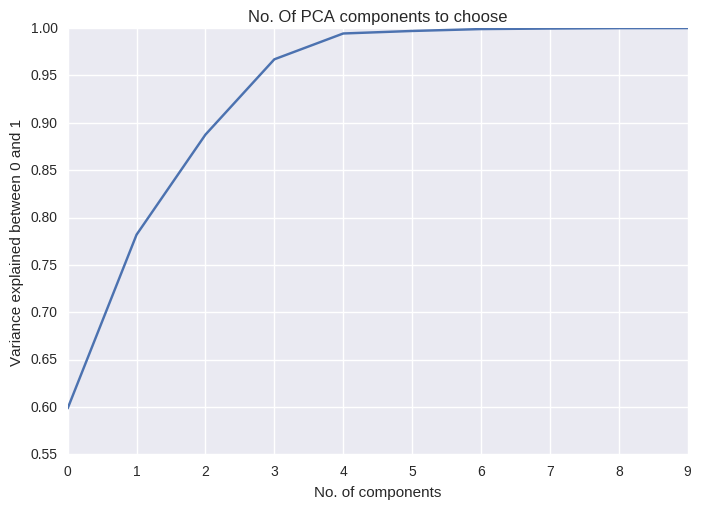
\includegraphics[totalheight=6cm]{PCA_number_of_elements_to_choose.png}}
    \caption{PCA Components}
    \label{fig:verticalcell}
\end{figure}

\subsection*{Prediction-Based Anomaly Detection}
The basis for prediction is an observed pattern and the assumption that it is reoccurring (with slight modifications) in the future. We assume our data follows a regular underlying pattern
and therefore also assume that the model describes the usual behavior well. Detecting anomalies using prediction follows this idea and is related to the statistical measure of residuals. Basically, this method predicts a value for each minute of the day by taking all previous measurement at the same time of the day. As an example, assume we predict the value for a Tuesday at 11:05am. We would now average all previous observed values of a Tuesday at 11:05am. Taking just an average would have the disadvantage of neglecting recent developments in the time series \cite{janetzko2014anomaly}. We therefore use a weighted averaging scheme with higher factors for recent values and linearly decreasing influence weights for older values. Further detailed explanations can be found in \cite{hao2011visual}.

After predicting for each point in a time series the expected values based on all values occurring before this point in the time series, we can compute the difference between predicted and observed values. The difference is an indicator for the abnormality of the point in a time series but needs for higher expressiveness some kind of normalization. From the choice and the design of the prediction method we are assuming a model which may not be applicable to all observed time series. We counterbalance for this fact by calculating the average fitting of our model. More in detail, we compute the average deviation from the predicted values for the whole time series. If a whole time series is highly unpredictable, the differences between predicted and actual values are less meaningful compared to a case when a time series follows perfect daily patterns with small deviations. Computation of the anomaly score is summarized by the following equation \cite{janetzko2014anomaly}:

anomaly[time] = $\frac{|predVal[time] - obsVal[time]|}{avgt∈Time (|predVal[t] - obsVal[t]|)}$\\

\subsection*{Clustering-Based Anomaly Detection}
\frenchspacing
The second approach for detecting anomalies in time series data is similarity-based. We assume often-observed patterns to be the usual behavior and rarely occurring patterns to be abnormal. Following this idea, we first have to define and compute the similarity of patterns in order to detect whether a pattern occurs more than once. The approach described in this section is proposed and presented by Bellala et al. in [\cite{bellala2012following},\cite{bellala2011towards}]. The time series is first partitioned into days and afterwards transformed by a Fourier transformation into the frequency domain. Each day of the time series is resulting in a k-dimensional vector in the frequency domain with k being a parameter of the transformation process. The next step described by Bellala et al. is a dimension reduction by multi-dimensional scaling into a two-dimensional space. The density distribution in the reduced MDS space is now interpreted as an anomaly score. Points (time series of a single day) being in a high-density area with many (similar) neighbors are assumed to reflect the usual behavior. Outliers in the 2D space can be seen as days with unusual values and are assigned a high anomaly score. This technique only takes the frequency domain into account and does not integrate external effects like weather data or week of the day.\\

 \subsection*{Gaussian Mixture Model-Based Anomaly Detection}
Here we propose yet another unsupervised algorithm for anomaly detection using Gaussian Mixture Model. The Gaussian Mixture Model(GMM) is used to model the probability density function of a feature vector, x, by the weighted combination of M multi-variate Gaussian densities $(\lambda)$ \cite{marinai2007machine} :
\begin{equation}\label{eq:1}
  p(x|\lambda)= \sum_{i=1}^{M} {p_ig_i(x)}  \\
 \end{equation}

First we fit a Gaussian Mixture Model (GMM) with Gaussians centered at each data point to a given data set. We then estimate the mixture proportion by applying Expectation Maximization algorithm to the given dataset. Each mixture proportion will represent the degree to which the point is a cluster center. The higher the mixture proportion, the more likely it is a cluster center, which means it has higher influence on other points. Reversely, the lower the mixture proportion is, the less likely the point is a cluster center, which means it has lower influence on other points. The outlier factor at each data point is then defined as a weighted sum of the mixture proportions with weights representing the similarities to other data points.	

\begin{figure}[tph!]
\centerline{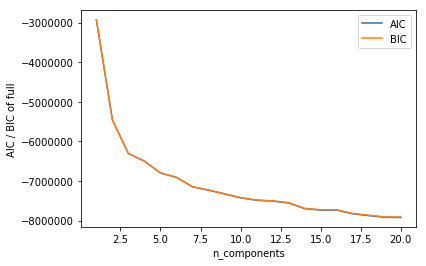
\includegraphics[totalheight=6cm]{BIC_1.png}}
    \caption{BIC score to determine the number of gaussians to choose}
    \label{fig:verticalcell}
\end{figure}
\label{sec:Algorithm}

Given a set of data points$ X ={x_1, . . . , x_n} $, a standard Gaussian mixture model clustering seeks to maximize the scaled log-likelihood function \cite{perl2009outlier}\\
\begin{equation}\label{eq:2}
  l(\pi_{1:m}, \mu_{1:m}, \lambda; X)= \frac{1}{n}\sum_{i=1}^{n} {log[\sum_{j=1}^{m}{\pi_ jp(x_i|\mu_j,\lambda)}]}  \\
 \end{equation}
 where m is the number of model components, $\pi_j = p(\omega_j |\lambda)$ represents the strength of jth component $\omega_j$ with $\sum_{i=1}^{m}{\pi_i = 1}$ and $\pi_{1:m}$ is a vector composed of $\pi_j$ for j = 1, . . . , m. The probability $p(x_i|\mu_j , \lambda)$ is a Gaussian and $\lambda$ is a vector of parameters specified below.

In the standard mixture model $\mu_j$ is the unknown mean vector for jth component and is estimated together with other parameters using an EM algorithm. Since our goal is not clustering but an estimation of an outlier factor at every data point, we assume that each data point is a cluster center. Thus, we set, m = n and $\mu_j = x_j$ for j = 1, . . . , n. This way, the
mixture proportion $\pi_j$ represents the likelihood of point $x_j$ to be a cluster center. We obtain a simplified version of Eq. (\ref{eq:2}):\\
\begin{equation}\label{eq:3}
  l(\pi_{1:m} ; X)= \frac{1}{n}\sum_{i=1}^{n} {log[\sum_{j=1}^{n}{\pi_ jp(x_i|x_j,\lambda)}]}  \\
 \end{equation}

In E-step we compute for each class i = 1, . . . , n and for each data point k = 1, . . . , n:
\begin{equation}\label{eq:4}
p(x_i|x_k,\lambda_t) = \frac{p(x_k|x_i,\lambda_t)p(x_i|\lambda_t)}{p(x_k|\lambda_t)} \\
= \frac{p(x_k|x_i)\pi_i(t)}{\sum_{j=1}^{n}{p(x_k|x_j)\pi_j(t)}}
\end{equation}

Our M-step is particularly simple, since we only need to update the mixture proportions:
\begin{equation}\label{eq:5}
\pi_j(t+1) = \frac{1}{n}\sum_{k=1}^{n}{p(x_i|x_k,\lambda_t)}
\end{equation}

Plugging in Eq. (\ref{eq:4}) in Eq. (\ref{eq:5}) gives
\begin{equation}\label{eq:6}
\pi_j(t+1) = \frac{1}{n}\sum_{k=1}^{n}{\frac{p(x_k|x_i)\pi_i(t)}{\sum_{j=1}^{n}{p(x_k|x_j)\pi_j(t)}}}
\end{equation}

the term $p(x_k|x_j)\pi_j(t)$ represents how much point $x_k$ is influenced by point $x_j$ with $p(x_k|x_j)$ being the strength of the connection and $\pi_j(t)$ measuring the importance of point j. This motivates the proposed definition of the outlier factor at point $x_k$ as
\begin{equation}\label{eq:7}
F_k = \sum_{j=1}^{n}{p(x_k|x_j)\pi_j(t)}
\end{equation}
According to Eq. (\ref{eq:7}), the smaller $F_k$, the more likely is data point $x_k$ to be an outlier.



\chapter{Implementating Anomaly Detection Mechanisms}
So far we have discussed the motivation and the algorithms proposed, to achieve the objectives of our thesis. This chapter will present the implementation details of the algorithms. All the implementation is done using python and its dependent machine learning libraries. We have experimented two different approaches in our work, one based on PCA residual space and other on Gaussian Mixture Models. The experiment is conducted in order to find positive and negative aspects with the two approaches proposed in order to make the final results as useful as possible.

We implemented our own anomaly injection tool which will insert the anomalies at any location in the data, user is given a choice of controlling the number of anomaly points and the choice of where to insert. The details will be explained below. We then show the details of PCA and GMM algorithm implementation details.
\\
\section{\textbf{Anomaly injection Tool}} 
\begin{figure}
\centerline{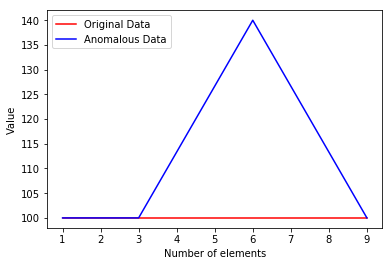
\includegraphics[totalheight=8cm]{anomaly-injection-identical-data.png}}
    \caption{Anomaly injection on an array containing all duplicate values. As an example this figure contains an array with all elements of the array having value '100'}
    \label{fig:ai_iden}
\end{figure}

We developed an anomaly injection tool to inject anomalies into our dataset to evaluate the accuracy of our anomaly detection methods. This tool manually injects anomalous data at any point of selection. We can even specify the number of anomalous points to inject, when we say injected anomalous points we mean, the existing data values are updated in such a way that the points represents values which looks unusual to the detection algorithms and the algorithms should be able to identify and classify them as anomalous. 

The developed tool has four parameters, \textbf{\textit{num}}, array containing the data, \textbf{\textit{x}}, is the parameter which lets the user to choose the percentage increase user wants to make to the data to look anomalous, \textbf{\textit{mid\_pos}}, the position in the data array where anomaly will be introduced, \textbf{\textit{count}}, will let the user control and keep count on the number of anomalies to put inside the data. One unique feature of this anomaly tool is, we do not need to introduce anomalies which looks obvious, instead, we have designed in such a way as to increase the value of selected point to  \textbf{\textit{x}}\% and additionally we provide the option to set the number of points to be made anomalous( \textbf{\textit{count}}). The count introduces those many anomaly points as the value itself on both sides of the selected point. 

The anomaly value is added to this range which follows a pattern of gradually increasing  from \textbf{\textit{mid\_pos}} - \textbf{\textit{count}} upto \textbf{\textit{mid\_pos}}  and then decreases gradually to   \textbf{\textit{mid\_pos}} + \textbf{\textit{count}} as shown in Fig \ref{fig:ai_iden} and  Fig \ref{fig:ai_rd}.  The distribution of original data and the anamolous data are plotted with simple line plot where x axis represents the index of the elements and y-axis represents the elements itself. The distribution in red depicts the behavior of unmodified elements and the distribution in blue depicts the behavior after injecting anamolies. Fig \ref{fig:ai_iden} shows the anomaly injection pattern for array containing all identical values and Fig \ref{fig:ai_rd} representing anomaly injection pattern for array containing random values. 

Two types of cases has been looked for in this area. One, all identical values elements and two, elements with random values. For identical values just for depicting the behavior of its distribution we used sample data and the results are shown in the Fig \ref{fig:ai_iden} and  Fig \ref{fig:ai_rd}. The point of insertion is at position 6 and number of anomaly points injected = 3 with the percentage of increase x=40\%, as you can see from Fig \ref{fig:ai_iden} the mid point at position 6 is increased 40\% (value = 140), either sides of it from position 3 to 6 and 6 to 9 are affected. Similarly to check with random data we used a list of random 10 numbers and injected 3 anomaly points on either sides from the selected middle point with x=40\%. We were successful in injecting the anomaly at the user provided point and range even for the random data as seen in the Fig \ref{fig:ai_rd}. 
\begin{figure}
\centerline{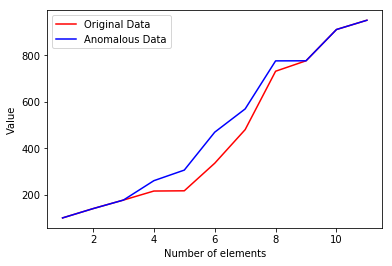
\includegraphics[totalheight=8cm]{anomaly-injection-random-data.png}}
    \caption{Anomaly injection on an array containing random data.}
    \label{fig:ai_rd}
\end{figure}

This anomaly injection tool can be used as a measure to check the accuracy of our methods. We know where we have injected the data and if the model is able to detect those anomalies which we have injected, then we can assure of a working anomaly detection method for our electrical data. With this tool in place we can also find out the number of false positives, false negatives, true positives as well as true negatives if any in our system. The design goal of this injection tool was mainly to evaluate the precision of our detection technique, to know how much deviation from the normal behavior can our model capture given the range of anomaly points. We assume our model to capture at least the mid point changes done while injecting the anomaly and nearby few points depending on the number of anomalies actually being injected.\\

At first, we take one week's Monday to Friday data and split it randomly into 80\% training data and remaining 20\% as the test data. We do not make any assumptions for supervised machine learning techniques here. The training and testing data are used with reference to unsupervised machine learning i.e the training set is composed of unmodified original datasets and the testing test is composed of modified datasets. The training set is used for modeling and learning our proposed algorithms, testing set is used to test the model(which are trained on the original dataset). Testing dataset will undergo anomaly injection procedure, to put few or may be more than few anomalous points. 

The anomaly injection tool is our own contribution to modify the datasets to contain abnormal values in a pre-defined fashion, the description of this tool is explained in Chapter 6. The percentage split is just random considering that the training dataset should be more than the testing dataset. We can choose anything between 50-50 split to 60-40, 70-30, or 80-20 depending on the size of the dataset. Since we have taken one week's data we want to capture most of the statistical values and hence decided to go with 80-20 split. We would also look into evaluating against 70-30 split in future or if the results are not as expected. For this we use the sklearn library's model\_selection.train\_test\_split() function which takes data and percentage variable ( which should be between 0 and 1) as parameters. The percentage variable if set to 0.5 gives us 50 percent training and 50 percent testing split of the data. Similarly, if the variable takes 0.6 then its a 60-40 split and so on. \\

\section{PCA residual space approach:}
PCA subspace projection is applied to data that have undergone random projection. Two key observations motivate this proposal. First, the computational complexity of PCA, when computed using the standard approach based on the singular value decomposition, scales like $O(l^3 + l^2n)$, where \textit{l} is the dimensionality of the data and \textit{n} is the sample size. Thus, use of the PCA subspace method is increasingly less feasible with the ever-increasing size and dimensions of modern data sets. Similar implementation has been already done in \cite{geijerlog}. 
\\
\section{GMM clustering approach:}

\label{sec:Impl}

\chapter{Evaluation}

In order to evaluate the performance and correctness of our proposed GMM and PCA-based anomaly detection methods, we have trained and tested the models against the set of data provided by \textbf{"PolyEnergyNet – Resiliente Polynetze zur sicheren Energieversorgung"}. We started the analysis by grouping the datasets into weekday and weekends in order to identify the patterns of these two groups separately. We believe the patterns to differ significantly between the weekday and weekends. 

At first, we take one week's Monday to Friday data and split it randomly into 80\% training data and remaining 20\% as the test data. We do not make any assumptions for supervised machine learning techniques here. The training and testing data are used with reference to unsupervised machine learning i.e the training set is composed of unmodified original datasets and the testing test is composed of modified datasets. The training set is used for modeling and learning our proposed algorithms, testing set is used to test the model(which are trained on the original dataset). Testing dataset will undergo anomaly injection procedure, to put few or may be more than few anomalous points. 

The anomaly injection tool is our own contribution to modify the datasets to contain abnormal values in a pre-defined fashion, the description of this tool is explained later in this section in detail. The percentage split is just random considering that the training dataset should be more than the testing dataset. We can choose anything between 50-50 split to 60-40, 70-30, or 80-20 depending on the size of the dataset. Since we have taken one week's data we want to capture most of the statistical values and hence decided to go with 80-20 split. We would also look into evaluating against 70-30 split in future or if the results are not as expected. For this we use the sklearn library's model\_selection.train\_test\_split() function which takes data and percentage variable ( which should be between 0 and 1) as parameters. The percentage variable if set to 0.5 gives us 50 percent training and 50 percent testing split of the data. Similarly, if the variable takes 0.6 then its a 60-40 split and so on. \\

\subsection*{\textbf{Anomaly injection Tool}} 
\begin{figure}
\centerline{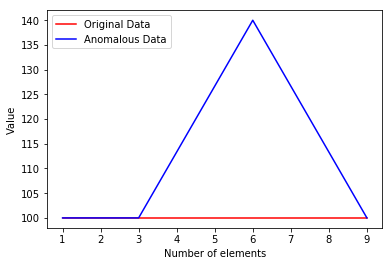
\includegraphics[totalheight=8cm]{anomaly-injection-identical-data.png}}
    \caption{Anomaly injection on an array containing all duplicate values. As an example this figure contains an array with all elements of the array having value '100'}
    \label{fig:ai_iden}
\end{figure}

We developed an anomaly injection tool to inject anomalies into our dataset to evaluate the accuracy of our anomaly detection methods. This tool manually injects anomalous data at any point of selection. We can even specify the number of anomalous points to inject, when we say injected anomalous points we mean, the existing data values are updated in such a way that the points represents values which looks unusual to the detection algorithms and the algorithms should be able to identify and classify them as anomalous. 

The developed tool has four parameters, \textbf{\textit{num}}, array containing the data, \textbf{\textit{x}}, is the parameter which lets the user to choose the percentage increase user wants to make to the data to look anomalous, \textbf{\textit{mid\_pos}}, the position in the data array where anomaly will be introduced, \textbf{\textit{count}}, will let the user control and keep count on the number of anomalies to put inside the data. One unique feature of this anomaly tool is, we do not need to introduce anomalies which looks obvious, instead, we have designed in such a way as to increase the value of selected point to  \textbf{\textit{x}}\% and additionally we provide the option to set the number of points to be made anomalous( \textbf{\textit{count}}). The count introduces those many anomaly points as the value itself on both sides of the selected point. 

The anomaly value is added to this range which follows a pattern of gradually increasing  from \textbf{\textit{mid\_pos}} - \textbf{\textit{count}} upto \textbf{\textit{mid\_pos}}  and then decreases gradually to   \textbf{\textit{mid\_pos}} + \textbf{\textit{count}} as shown in Figure \ref{fig:ai_iden} and  Figure \ref{fig:ai_rd}.  The distribution of original data and the anamolous data are plotted with simple line plot where x axis represents the index of the elements and y-axis represents the elements itself. The distribution in red depicts the behavior of unmodified elements and the distribution in blue depicts the behavior after injecting anamolies. Figure \ref{fig:ai_iden} shows the anomaly injection pattern for array containing all identical values and Figure \ref{fig:ai_rd} representing anomaly injection pattern for array containing random values. 

Two types of cases has been looked for in this area. One, all identical values elements and two, elements with random values. For identical values just for depicting the behavior of its distribution we used sample data and the results are shown in the Figures \ref{fig:ai_iden} and  Figure \ref{fig:ai_rd}. The point of insertion is at position 6 and number of anomaly points injected = 3 with the percentage of increase x=40\%, as you can see from figure \ref{fig:ai_iden} the mid point at position 6 is increased 40\% (value = 140), either sides of it from position 3 to 6 and 6 to 9 are affected. Similarly to check with random data we used a list of random 10 numbers and injected 3 anomaly points on either sides from the selected middle point with x=40\%. We were successful in injecting the anomaly at the user provided point and range even for the random data as seen in the figure \ref{fig:ai_rd}. 
\begin{figure}
\centerline{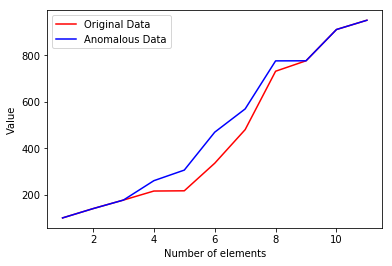
\includegraphics[totalheight=8cm]{anomaly-injection-random-data.png}}
    \caption{Anomaly injection on an array containing random data.}
    \label{fig:ai_rd}
\end{figure}

This anomaly injection tool can be used as a measure to check the accuracy of our methods. We know where we have injected the data and if the model is able to detect those anomalies which we have injected, then we can assure of a working anomaly detection method for our electrical data. With this tool in place we can also find out the number of false positives, false negatives, true positives as well as true negatives if any in our system. The design goal of this injection tool was mainly to evaluate the precision of our detection technique, to know how much deviation from the normal behavior can our model capture given the range of anomaly points. We assume our model to capture at least the mid point changes done while injecting the anomaly and nearby few points depending on the number of anomalies actually being injected.



\begin{enumerate}
\item\textbf{PCA}

We start the evaluation of PCA based anomaly detection method by briefly specifying the steps involved in preprocessing and then dive into describing the performance of our PCA based anomaly detection method. The preprocessing for PCA based anomaly detection will be done as follows:
\begin{itemize}
\item\textbf{Data Smoothing:} In order to clearly reveal the underlying trends and seasonal variations of our time series data we apply the simple "moving average" as our data smoothing method. This moving average will smooth the random variation or we can say, the noise in the data by taking average of values over the given window period. Moving average works better when using data which are measured equi-distantly, by equi-distantly we mean, all the observations are taken at equal time intervals i.e every second data. We use window size = 60 which corresponds to one minute of our data. All the variations such as for example, a sudden dip in the phase displacement(CosPhi value) which might have occured due to incorrect sensor readings will be smoothed.

\item\textbf{Normalization:} The smoothed data is normalized by removing the mean of each column and the difference to mean is stored as the normalized value. What we are doing here is scaling the values of each column of our dataset to represent mean 0 and unit variance. Our data contains columns such as voltages, current, power, phase displacement values and these values are not measured against a single unit, that is, voltage values are in Volts, current values are in Amperes, power values are in Watt-hour and phase displacement are in Degrees. If we do not normalize this data then the result of PCA for choosing the right number of components will not be accurate. By right number of components we mean that the components may represent variances captured by columns which contain larger values. In our dataset we see that, power values are in the range of thousands to hundreds of thousands, voltages are in range of 200 to 270, current are within 100 to 150, where as phase displacement values are within 1. 

Without normalizing we tend to obtain components of largest values like variances of  power and/or voltages  as high variance since their values are very large and the phase displacement values which are too low can be neglected. To account for this, we scaled the values such that each column had mean of 0 and variance of 1, this ensured that the variance in all the columns are retained and made sure PCA will consider all the necessary features and thus the components we choose after applying PCA were correct when it comes to identifying the right number of components.

\item\textbf{Extracting relevant features:} Once the data is smoothed and normalized, the next step we carried out was to divide all the features based on the amount of variances captured by applying PCA . Our aim here was to group the features into two subgroups which we call as normal subspace and residual subspace. Normal subspace is composed of components capturing the major variances and residual subspace is composed of components capturing the minor variance which are usually ignored. Our contribution will be researching in this residual subspace as we assume any anomalous data will be captured by this residual subspace and then we define a threshold value above which, we term the data points as tagged as anomalous points. 
   
\begin{figure}
\centerline{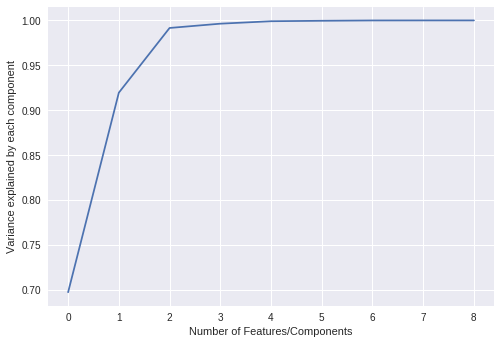
\includegraphics[totalheight=8cm]{PCA_cusum_variance.png}}
    \caption{Cumulative Sum of PCA explained variance.}
    \label{fig:PCA_cusum_variance}
\end{figure}

\item\textbf{Threshold:} An optimal threshold is defined to distinguish between normal and anomalous data. As discussed earlier while describing our PCA based anomaly detection method, we define a threshold value derived from calculating Squared Prediction Error. All the values above this threshold are considered as anomalies. 

\item\textbf{Results:} We fit the PCA model for all the 9 columns of our data and transform our data to PCA axes. The resultant PCA model divided the data into two orthogonal subspaces namely, normal subspace and residual subspace. Normal subspace is constituted of 'n' components based on the percentage of variance we wish to retain. The percentage of variances are nothing but the eigen values of the corresponding n components. The results of fitting our data with PCA is better explained by the measure "cumulative sum of explained variance ratio" as shown in the Figure \ref{fig:PCA_cusum_variance}. From the figure, we can explain the variances of all components. Component 0 which is the first component captures 70\% of the variance or has the largest eigen value, component 1 together with component 0 captures about 91.9\% variance, component 2 added  to the first two will account for 99.1\% and so on. 
\begin{figure}
\centerline{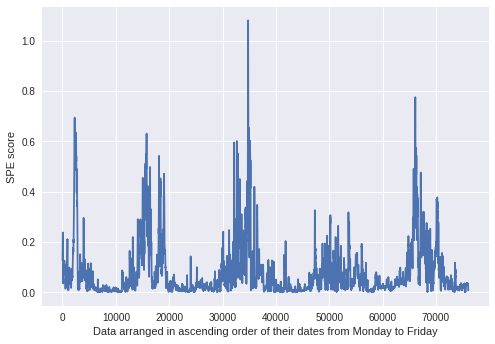
\includegraphics[totalheight=8cm]{SPE_error.png}}
    \caption{Results of SPE Error value against the data}
    \label{fig:spe}
\end{figure}
We had to play around with our experiments to come up with the right amount of residual space taking into consideration how much variances should we capture in normal subspace and how much variance should be allowed to retain in residual subspace. We evaluated starting from two components explaining 91.9\% through five components explaining 99.9\% of variance.
\end{itemize}

\item\textbf{GMM}

We follow a similar procedure as we followed for PCA based approach. The GMM based anomaly detection results when compared to PCA based methods were quite satisful and we were able to detect both the injected anomalies and the unusual behavioral data in our dataset.

\begin{itemize}
\item\textbf{Dataset and preprocessing:} We took same one weeks data from Monday to Friday which we used for PCA as well. This data was subjected to filtering and data smoothing similar to the steps followed under PCA. In order to account for equal variability the dataset had to undergo dimensionality reduction for which we used the principal component analysis. From the variance explained by each component we made a decision to use first three prinicpal components which were able to capture 99.9\% variance as can be seen in the Figure \ref{fig:PCA_cusum_variance}.

\begin{figure}
\centerline{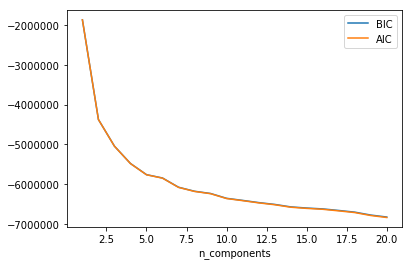
\includegraphics[totalheight=8cm]{BIC_AIC.png}}
    \caption{BIC score for the data}
    \label{fig:bic}
\end{figure}

\item\textbf{Model the data:} The data was fitted using the Gaussian Mixture Model function readily available with the python package of scikit learn. To efficiently model our data and to understand the underlying behavior using GMM, we had to carefully choose the fitting parameters. We measure the correctness and the perfectness of our model by carefully looking at,  the \textit{number of clusters}. 

Cluster number will determine how well our GMM will fit our data. GMM uses the Expectation-Maximization algorithm as described earlier in our work to assign data points to the clusters. If the clusters are too less, then the model will underfit the data constraining all the data points into these small clusters and if the number of cluster is too high, then data which are closely related could be placed in different clusters leading to overfitting of the data. To handle this condition of overfitting and underfitting we use Bayesian Information Criterion(BIC) score to estimate the right number of clusters. We chose 50 as the initial cluster number and gradually reduced in steps of 10 keeping in my mind of the overfitting criteria and finally came down to use 20 as the number of clusters to GMM which is as shown in the Figure \ref{fig:bic}.

\begin{figure}
\centerline{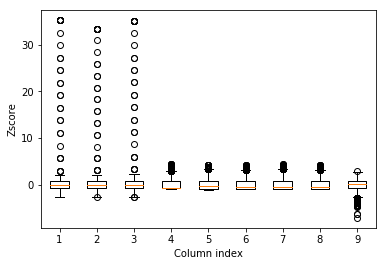
\includegraphics[totalheight=8cm]{Boxplot_Zscore.png}}
    \caption{BIC score for the data}
    \label{fig:bic_zs}
\end{figure}
\item\textbf{Results:} The results obtained using GMM on our electrical data is visualized in Figure \ref{fig:bic_zs} and Figure \ref{fig:ss}. Figure \ref{fig:bic_zs} visually illustrate many points outside the boxplot's inter-quartile range with unfilled circles. These points are clearly anomalous in nature compared to other data points which fall within inter-quartile range. The unfilled circles formed by the unusual data points are results of injecting anomalies into our data using the anomaly tool developed and described earlier. For our model to perform better it should be able to identify these injected points and classify them as anomalous. 

The score samples are the measure of weighted log probabilities of the data points obtained after fitting the test data injected with anomalies to GMM. The points are plotted in the form of histogram as expressed by Figure \ref{fig:ss}. We calculate the confidence intervals from the obtained score sample values of each data point. With the assumption of data following Gaussian distribution, we go by defining an optimal threshold value based on percentage of confidence intervals we wish to retain and standard deviation measure.

We considered weighted log probabilities or score samples as a measure to distinguish between normal data and abnormal data. Normal data are the points which have high score sample values, that is values closer to 0 and all the points which tend to move away from 0 have very low probability score. Thereby limiting these low probability values to be equal to some threshold, we derive a margin and say all the points falling above this margin as anomalous. 

Carefully defining the threshold was the main aim after we have our model ready for detection. We incorporate some of the important statistical measures for our needs to explain the threshold value, such as confidence intervals, standard deviations. In common statistical process, we consider 3 standard deviation's value, collectively representing 99.73\% of points belonging to normal distribution. Here as well in our work, we use standard deviation value and tweak its value to obtain the best threshold which can easily distinguish between points of low and high probabilities.

With 2.5 times standard deviation and confidence interval of 95\% we obtained a threshold value equal to 11.099 which was sufficient enough to determine and detect the value as anomaly. Our test data had 76000 observations and without any injections we found to have 81 points which our model detected as anomalous points. These points which were detected may be caused due to faulty measurements occurred while reading the electrical units. We assume it to be faulty because the measured values when we inspected manually were found to be very unusual such as very low phase displacement values(CosPhi is the column name in our dataset), without change in any other columns(like voltages or current or power).

From now on, everytime we calculate the count of number of anomalies detected by our model to be the count as result calculated currently minus 81 which we saw in the original dataset. We inserted anomalies manually as well as with our injection tool. With the manual injection we were able to detect all the manually injected anomalies, this was obvious since we had changed the voltages and current units to a value which looks really obvious to anyone looking at the data itself. So we are happy with the first step of detection process in obvious looking anomalies. The next step was to insert anomalies with our injection tool. We started with initial injection of only few points in the range of 10 and with an increase of  40\% to the midpoint chosen as the point of injection. We remind you, the anomalies are inserted on either side of this mean point, count will determine the number of points on either side of mean is affected and the share of these points are with respect to the mid point.

The results show that our method were able to efficiently detect these points as well. The detection was not 100\% since the values are increased with a pattern as discussed previously, that is the value increases slowly upto the mean and gradually decreases after the mean. Since there is only small variation to the data points which are at the extreme ends of the point chosen for insertion, we believed our model to not detect these points. And fortunately, we were able to detect the points which were closer to the extreme ends, infact 6 to 8 observations out of 10 were detected with confidence intervals of 95\% and standard deviation of 2.5. 
\begin{figure}
\centerline{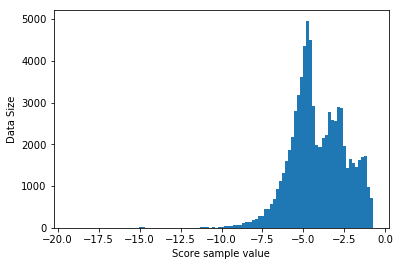
\includegraphics[totalheight=8cm]{Score_samples.png}}
    \caption{BIC score for the data}
    \label{fig:ss}
\end{figure}

\end{itemize}

\end{enumerate}

\label{sec:Eval}

\chapter{Conclusion and Future Work}
\label{sec:Conclusion}

%\cleardoublepage

\refstepcounter{dummy}
\listoffigures
	
\refstepcounter{dummy}
\listoftables
	
\refstepcounter{dummy}
	
\bibliographystyle{plain}	
\bibliography{thesis}{}

\end{document}          

